\flushbottom










%%============================================================================
%%============================================================================
\chapter{Regular Sturm-Liouville Problems}
\index{regular Sturm-Liouville problems}



\begin{tabbing}
  I learned there are troubles \\
  Of more than one kind. \\
  Some come from ahead \\
  And some come from behind. \\
  \\
  But I've bought a big bat. \\
  I'm all ready, you see. \\
  Now my troubles are going \\
  To have troubles with \textit{me}!
\end{tabbing}

\begin{flushright}
  -\textit{I Had Trouble in Getting to Solla Sollew}\\
  -Theodor S. Geisel, (Dr. Suess)
\end{flushright}










%%============================================================================
\section{Derivation of the Sturm-Liouville Form}



Consider the eigenvalue problem on the finite interval $[a \ldots b]$,
\[ 
p_2(x) y'' + p_1(x) y' + p_0(x) y = \mu y,
\]
subject to the homogeneous unmixed boundary conditions
\[ 
\alpha_1 y(a) + \alpha_2 y'(a) = 0, \qquad
\beta_1 y(b) + \beta_2 y'(b) = 0. 
\]
Here the coefficient functions $p_j$ are real and continuous 
and $p_2 > 0$ on the interval $[a \ldots b]$.  
(Note that if $p_2$ were negative we could multiply the equation by
$(-1)$ and replace $\mu$ by $-\mu$.)
The parameters $\alpha_j$ and $\beta_j$ are real.

We would like to write this problem in a form that can be used to obtain
qualitative information about the problem.  First we will write the
operator in self-adjoint form.  We divide by $p_2$ since it is non-vanishing.
\[
y'' + \frac{p_1}{p_2} y' + \frac{p_0}{p_2} y = \frac{\mu}{p_2} y.
\]
We multiply by an integrating factor.
\[
\]
\begin{gather*}
  I = \exp \left( \int \frac{p_1}{p_2}\,\dd x \right) \equiv \e^{P(x)}
  \\
  \e^{P(x)} \left( y'' + \frac{p_1}{p_2} y' + \frac{p_0}{p_2} y
  \right) = \e^{P(x)} \frac{\mu}{p_2} y 
  \\
  \left( \e^{P(x)} y' \right)' + \e^{P(x)} \frac{p_0}{p_2} y  = \e^{P(x)} \frac{\mu}{p_2} y
\end{gather*}

For notational convenience, we define new coefficient functions and parameters.
\[ 
p = \e^{P(x)}, \quad 
q = \e^{P(x)} \frac{p_0}{p_2}, \quad
\sigma = \e^{P(x)} \frac{1}{p_2}, \quad
\lambda = -\mu.
\]
Since the $p_j$ are continuous and $p_2$ is positive, $p$, $q$, and $\sigma$
are continuous.  $p$ and $\sigma$ are positive functions.
The problem now has the form,
\[ 
(p y')' + q y + \lambda \sigma y = 0,
\]
subject to the same boundary conditions,
\[ 
\alpha_1 y(a) + \alpha_2 y'(a) = 0, \qquad
\beta_1 y(b) + \beta_2 y'(b) = 0. 
\]
This is known as a \textit{Regular Sturm-Liouville} problem.  
We will devote 
much of this chapter to studying the properties of this problem.  We will
encounter many results that are analogous to the properties of 
self-adjoint eigenvalue problems.






\begin{Example}
  \[ 
  \frac{\dd}{\dd x}\left( \ln x \frac{\dd y}{\dd x}\right) + \lambda x y = 0,
  \qquad y(1) = y(2) = 0
  \]
  is not a regular Sturm-Liouville problem since $\ln x$ vanishes at $x = 1$.
\end{Example}





\begin{Result}
  Any eigenvalue problem of the form
  \begin{gather*}
    p_2 y'' + p_1 y' + p_0 y = \mu y, \quad \mathrm{for}\ a \leq x \leq b,
    \\
    \alpha_1 y(a) + \alpha_2 y'(a) = 0, \quad \beta_1 y(b) + \beta_2 y'(b) = 0,
  \end{gather*}
  where the $p_j$ are real and continuous and $p_2 > 0$ on $[a,b]$, and 
  the $\alpha_j$ and $\beta_j$ are real can be written in the form of a regular 
  Sturm-Liouville problem,
  \begin{gather*}
    (p y')' + q y + \lambda \sigma y = 0, \quad \mathrm{on}\ a \leq x \leq b, 
    \\
    \alpha_1 y(a) + \alpha_2 y'(a) = 0, \quad \beta_1 y(b) + \beta_2 y'(b) = 0.
  \end{gather*}
\end{Result}









%%============================================================================
\section{Properties of Regular Sturm-Liouville Problems}

\paragraph{Self-Adjoint.}
Consider the Regular Sturm-Liouville equation.
\[ 
L[y] \equiv (p y')' + q y = - \lambda \sigma y.
\]
We see that the operator is formally self-adjoint.  Now we determine if the 
problem is self-adjoint.
\begin{align*}
  \langle v | L[u] \rangle - \langle L[v] | u \rangle 
  &= \langle v | (p u')' + q u \rangle - \langle (p v')' + q v | u \rangle 
  \\
  &= [ \overline{v} p u']_a^b - \langle \overline{v}' | p u' \rangle + \langle \overline{v} | q u \rangle
  - [p \overline{v}' u]_a^b + \langle p \overline{v}' | u' \rangle - \langle q \overline{v} | u \rangle 
  \\
  &= [ \overline{v} p u']_a^b - [p \overline{v}' u]_a^b 
  \\
  &= p(b) \big( \overline{v}(b) u'(b) - \overline{v}'(b) u(b) \big)
  + p(a) \big( \overline{v}(a) u'(a) - \overline{v}'(a) u(a) \big) 
  \\
  &= p(b) \left( \overline{v}(b) \left(-\frac{\beta_1}{\beta_2}\right) u(b) 
    - \left(-\frac{\beta_1}{\beta_2}\right)\overline{v}(b) u(b) \right)
  \\
  &\qquad + p(a) \left( \overline{v}(a) 
    \left(-\frac{\alpha_1}{\alpha_2}\right) u(a) 
    - \left(-\frac{\alpha_1}{\alpha_2}\right)
    \overline{v}(a) u(a) \right) 
  \\
  &= 0    
\end{align*}
Above we used the fact that the $\alpha_i$ and $\beta_i$ are real.
\[
\overline{ \left( \frac{\alpha_1}{\alpha_2} \right) } 
=  \left( \frac{\alpha_1}{\alpha_2} \right) , \qquad
\overline{ \left( \frac{\beta_1}{\beta_2} \right) }
= \left( \frac{\beta_1}{\beta_2} \right)
\]
Thus $L[y]$ subject to the boundary conditions is self-adjoint.







\paragraph{Real Eigenvalues.}
Let $\lambda$ be an eigenvalue with the eigenfunction $\phi$.  We start
with Green's formula.
\begin{gather*}
  \langle \phi | L[\phi] \rangle - \langle L[\phi] | \phi \rangle = 0 
  \\
  \langle \phi | - \lambda \sigma \phi \rangle - \langle - \lambda \sigma \phi | \phi \rangle = 0 
  \\
  - \lambda \langle \phi | \sigma | \phi \rangle + \overline{\lambda} \langle \phi | \sigma | \phi \rangle = 0 
  \\
  (\overline{\lambda} - \lambda) \langle \phi | \sigma | \phi \rangle = 0
\end{gather*}
Since $\langle \phi | \sigma | \phi \rangle > 0$, $\overline{\lambda} - \lambda = 0$.
Thus the eigenvalues are real.









\paragraph{Infinite Number of Eigenvalues.}
There are an infinite of eigenvalues which have no finite cluster point.
This result is analogous to the result that we derived for self-adjoint 
eigenvalue problems.  When we cover the Rayleigh quotient, we will find
that there is a least eigenvalue.  Since the eigenvalues are distinct and
have no finite cluster point, $\lambda_n \to \infty$ as $n \to \infty$.
Thus the eigenvalues form an ordered sequence,
\[ 
\lambda_1 < \lambda_2 < \lambda_3 < \cdots. 
\]










\paragraph{Orthogonal Eigenfunctions.}
Let $\lambda$ and $\mu$ be two distinct eigenvalues with the eigenfunctions
$\phi$ and $\psi$.  Green's formula states
\begin{gather*}
  \langle \psi | L[\phi] \rangle - \langle L[\psi] | \phi \rangle = 0. 
  \\
  \langle \psi | - \lambda \sigma \phi \rangle - \langle - \mu \sigma \psi | \phi \rangle = 0
  \\
  -\lambda \langle \psi | \sigma | \phi \rangle + \overline{\mu} \langle \psi | \sigma | \phi \rangle = 0 
  \\
  (\mu - \lambda) \langle \psi | \sigma | \phi \rangle = 0 
\end{gather*}
Since the eigenvalues are distinct, $\langle \psi | \sigma | \phi \rangle = 0$.
Thus eigenfunctions corresponding to distinct eigenvalues are orthogonal
with respect to $\sigma$.











\paragraph{Unique Eigenfunctions.}
Let $\lambda$ be an eigenvalue.  Suppose $\phi$ and $\psi$ are two independent
eigenfunctions corresponding to $\lambda$.  
\[
L[\phi] + \lambda \sigma \phi = 0,
\quad
L[\psi] + \lambda \sigma \psi = 0
\]
We take the difference of $\psi$ times the first equation and $\phi$ times 
the second equation.
\begin{gather*}
  \psi L[\phi] - \phi L[\psi] = 0 
  \\
  \psi (p \phi')' - \phi (p \psi')' = 0 
  \\
  (p (\psi \phi' - \psi' \phi))' = 0 
  \\
  p (\psi \phi' - \psi' \phi) = \mathrm{const}
\end{gather*}
In order to satisfy the boundary conditions, the constant must be zero.
\[ 
p (\psi \phi' - \psi' \phi) = 0 
\]
Since $p > 0$ the second factor vanishes.
\begin{gather*}
  \psi \phi' - \psi' \phi = 0 
  \\
  \frac{\phi'}{\psi} - \frac{\psi' \phi}{\psi^2} = 0 
  \\
  \frac{\dd}{\dd x} \left( \frac{\phi}{\psi} \right) = 0 
  \\
  \frac{\phi}{\psi} = \mathrm{const}
\end{gather*}
$\phi$ and $\psi$ are not independent.  Thus each eigenvalue has a 
unique, (to within a multiplicative constant), eigenfunction.






\paragraph{Real Eigenfunctions.}
If $\lambda$ is an eigenvalue with eigenfunction $\phi$, then
\[ 
(p \phi')' + q \phi + \lambda \sigma \phi = 0.
\]
We take the complex conjugate of this equation.
\[ 
\left(p \overline{\phi}' \right)' + q \overline{\phi} + \lambda \sigma \overline{\phi} = 0.
\]
Thus $\overline{\phi}$ is also an eigenfunction corresponding to $\lambda$.  Are 
$\phi$ and $\overline{\phi}$ independent functions, or do they just differ
by a multiplicative constant?  (For example, $\e^{\imath x}$ and $\e^{-\imath x}$ are
independent functions, but $\imath x$ and $- \imath x$ are dependent.)
From our argument on unique eigenfunctions, we see that
\[ 
\phi = (\mathrm{const}) \overline{\phi}. 
\]
Since $\phi$ and $\overline{\phi}$ only differ by a multiplicative constant, 
the eigenfunctions can be chosen so that they are real-valued functions.







\paragraph{Rayleigh's Quotient.}
\index{Rayleigh's quotient}
Let $\lambda$ be an eigenvalue with the eigenfunction $\phi$.
\begin{gather*}
  \langle \phi | L[\phi] \rangle = \langle \phi | - \lambda \sigma \phi \rangle 
  \\
  \langle \phi | (p \phi')' + q \phi \rangle = - \lambda \langle \phi | \sigma | \phi \rangle 
  \\
  \left[\overline{\phi} p \phi' \right]_a^b - \langle \phi' | p | \phi' \rangle + \langle \phi | q | \phi \rangle
  = - \lambda \langle \phi | \sigma | \phi \rangle 
  \\
  \boxed{ 
    \lambda = \frac{ -\big[p \overline{\phi} \phi' \big]_a^b + \langle \phi' | p | \phi' \rangle 
      - \langle \phi | q | \phi \rangle}
    { \langle \phi | \sigma | \phi \rangle }
    }
\end{gather*}
This is known as \textit{Rayleigh's quotient}.  It is useful for obtaining
qualitative information about the eigenvalues.











\paragraph{Minimum Property of Rayleigh's Quotient.}
\index{Rayleigh's quotient!minimum property}
Note that since $p$, $q$, $\sigma$ and $\phi$ are bounded functions,
the Rayleigh quotient is bounded below.  Thus there is a least eigenvalue.
If we restrict $u$ to be a real continuous function that satisfies the 
boundary conditions, then
\[ 
\lambda_1 = \min_u \frac{-[p u u']_a^b + \langle u' | p | u' \rangle - \langle u | q | u \rangle}{\langle u | \sigma | u \rangle},
\]
where $\lambda_1$ is the least eigenvalue.
This form allows us to get upper and lower bounds on $\lambda_1$.  

To derive this formula, we first write it in terms of the operator $L$.
\[ 
\lambda_1 = \min_u \frac{-\langle u | L[u] \rangle}{\langle u | \sigma | u \rangle}
\]
Since $u$ is continuous and satisfies the boundary conditions, we can 
expand $u$ in a series of the eigenfunctions.
\begin{align*}
  -\frac{\langle u | L[u] \rangle}{\langle u | \sigma | u \rangle}
  &= - \frac{\left\langle \sum_{n = 1}^\infty c_n \phi_n \big| L \left[ 
        \sum_{m = 1}^\infty c_m \phi_m \right] \right\rangle}
  {\left\langle \sum_{n = 1}^\infty c_n \phi_n \big| \sigma \big|
      \sum_{m = 1}^\infty c_m \phi_m \right\rangle} 
  \\
  &= - \frac{\left\langle \sum_{n = 1}^\infty c_n \phi_n \big|  
      -\sum_{m = 1}^\infty c_m \lambda_m \sigma \phi_m \right\rangle}
  {\left\langle \sum_{n = 1}^\infty c_n \phi_n \big| \sigma \big|
      \sum_{m = 1}^\infty c_m \phi_m \right\rangle} 
  \\
  \intertext{We assume that we can interchange summation and integration.}
  &= \frac{ \sum_{n = 1}^\infty \sum_{m = 1}^\infty \overline{c_n} c_m \lambda_n \langle \phi_m | \sigma | \phi_n \rangle}
  {\sum_{n = 1}^\infty \sum_{m = 1}^\infty \overline{c_n} c_m \langle \phi_m | \sigma | \phi_n \rangle} 
  \\
  &= \frac{\sum_{n = 1}^\infty |c_n|^2 \lambda_n \langle \phi_n | \sigma | \phi_n \rangle}
  {\sum_{n = 1}^\infty |c_n|^2 \langle \phi_n | \sigma | \phi_n \rangle} 
  \\
  &\leq \lambda_1 \frac{\sum_{n = 1}^\infty |c_n|^2 \langle \phi_n | \sigma | \phi_n \rangle}
  {\sum_{n = 1}^\infty |c_n|^2 \langle \phi_n | \sigma | \phi_n \rangle} 
  \\
  &= \lambda_1
\end{align*}
We see that the minimum value of Rayleigh's quotient is $\lambda_1$.  The minimum
is attained when $c_n = 0$ for all $n \geq 2$, that is, when $u = c_1 \phi_1$.








\paragraph{Completeness.}
The set of the eigenfunctions of a regular Sturm-Liouville problem is 
complete.  That is, any piecewise continuous function defined on $[a,b]$
can be expanded in a series of the eigenfunctions,
\[ 
f(x) \sim \sum_{n=1}^\infty c_n \phi_n(x),
\]
where the $c_n$ are the generalized Fourier coefficients,
\[ 
c_n = \frac{\langle \phi_n | \sigma | f \rangle}{\langle \phi_n |\sigma | \phi_n \rangle}.
\]
Here the sum is convergent in the mean.  For any fixed $x$, the sum
converges to $\frac{1}{2} (f(x^-) + f(x^+))$.
If $f(x)$ is continuous and satisfies the boundary conditions,
then the convergence is uniform.






\begin{Result}
  \label{sl_prop}
  \index{regular Sturm-Liouville problems!properties of}
  Properties of regular Sturm-Liouville problems.
  \begin{itemize}
  \item   
    The eigenvalues $\lambda$ are real.
  \item   
    There are an infinite number of eigenvalues
    \[ \lambda_1 < \lambda_2 < \lambda_3 < \cdots.\]
    There is a least eigenvalue $\lambda_1$ but there is no greatest eigenvalue,
    ($\lambda_n \to \infty$ as $n \to \infty$).
  \item   
    For each eigenvalue, there is one unique, (to within a multiplicative
    constant), eigenfunction $\phi_n$.  The eigenfunctions can be chosen to be
    real-valued.  (Assume the $\phi_n$ following are real-valued.)
    The eigenfunction $\phi_n$ has exactly $n-1$ zeros in the open interval
    $a < x < b$. 
  \item   
    The eigenfunctions are orthogonal with respect to the weighting
    function $\sigma(x)$.
    \[ 
    \int_a^b \phi_n(x) \phi_m(x) \sigma(x)\,\dd x = 0 \quad \mathrm{if}\ n \neq m.
    \]
  \item   
    The eigenfunctions are complete.  Any piecewise continuous function
    $f(x)$ defined on $a \leq x \leq b$ can be expanded in a series of 
    eigenfunctions
    \[ 
    f(x) \sim \sum_{n = 1}^\infty c_n \phi_n(x),
    \]
    where
    \[ 
    c_n = \frac{\int_a^b f(x) \phi_n(x) \sigma(x)\,\dd x}{\int_a^b \phi_n^2(x) \sigma(x)\,\dd x}.
    \]
    The sum converges to $\frac{1}{2}(f(x^-) + f(x^+))$.
  \item   
    The eigenvalues can be related to the eigenfunctions with a formula
    known as the Rayleigh quotient.
    \[ 
    \lambda_n = \frac{ - p \phi_n \frac{\dd \phi_n}{\dd x} \Big|_a^b
      + { \displaystyle \int_a^b }
      \left( p \left(\frac{\dd \phi_n}{\dd x}\right)^2 - q \phi_n^2
      \right)\,\dd x}
    {\int_a^b \phi_n^2 \sigma\,\dd x}
    \]
  \end{itemize}
\end{Result}




\begin{Example}
  \index{Fourier sine series}
  A simple example of a Sturm-Liouville problem is
  \[ 
  \frac{\dd}{\dd x}\left(\frac{\dd y}{\dd x}\right) + \lambda y = 0, \qquad
  y(0) = y(\pi) = 0.
  \]

  \paragraph{Bounding The Least Eigenvalue.}
  The Rayleigh quotient for the first eigenvalue is
  \[ 
  \lambda_1 = \frac{\int_0^\pi (\phi_1')^2 \,\dd x}{\int_0^\pi \phi_1^2 \,\dd x}. 
  \]
  Immediately we see that the eigenvalues are non-negative.  If 
  $\int_0^\pi (\phi_1')^2\,\dd x = 0$ then $\phi = (\mathrm{const})$.  
  The only constant that 
  satisfies the boundary conditions is $\phi = 0$.  
  Since the trivial solution is not an
  eigenfunction, $\lambda = 0$ is not an eigenvalue.  
  Thus all the eigenvalues are positive.

  Now we get an upper bound for the first eigenvalue.
  \[ 
  \lambda_1 = \min_u \frac{\int_0^\pi (u')^2 \,\dd x}{\int_0^\pi u^2\,\dd x} 
  \]
  where $u$ is continuous and satisfies the boundary conditions.  We choose
  $u = x (x - \pi)$ as a trial function.
  \begin{align*}
    \lambda_1
    &\leq \frac{\int_0^\pi (u')^2 \,\dd x}{\int_0^\pi u^2\,\dd x} 
    \\
    &= \frac{\int_0^\pi (2x-\pi)^2 \,\dd x}{\int_0^\pi (x^2-\pi x)^2 \,\dd x} 
    \\
    &= \frac{\pi^3 /3}{\pi^5 / 30} 
    \\
    &= \frac{10}{\pi^2} 
    \\
    &\approx 1.013
  \end{align*}

  \paragraph{Finding the Eigenvalues and Eigenfunctions.}
  We consider the cases of negative, zero, and positive eigenvalues to 
  check our results above.
  \begin{description}
  \item{$\mathbf{\boldsymbol{\lambda} \boldsymbol{<} 0}$.}
    The general solution is
    \[ 
    y = c \e^{\sqrt{-\lambda} x} + d \e^{- \sqrt{-\lambda} x}.
    \]
    The only solution that satisfies the boundary conditions is the trivial
    solution, $y = 0$.  Thus there are no negative eigenvalues.
  \item{$\mathbf{\boldsymbol{\lambda} \boldsymbol{=} 0}$.}
    The general solution is
    \[ 
    y = c + d x.
    \]
    Again only the trivial solution satisfies the boundary conditions, so
    $\lambda = 0$ is not an eigenvalue.
  \item{$\mathbf{\boldsymbol{\lambda} \boldsymbol{>} 0}$.}
    The general solution is
    \[ 
    y = c \cos(\sqrt{\lambda x}) + d \sin(\sqrt{\lambda} x).
    \]
    We apply the boundary conditions.
    \begin{alignat*}{2}
      y(0) &= 0 \qquad &\to \qquad &c = 0 \\
      y(\pi) &= 0 \qquad &\to \qquad &d \sin(\sqrt{\lambda} \pi) = 0 
    \end{alignat*}
    The nontrivial solutions are
    \[ 
    \sqrt{\lambda} = n = 1, 2, 3, \ldots \qquad y = d \sin(n \pi).
    \]
  \end{description}
  Thus the eigenvalues and eigenfunctions are
  \[ 
  \lambda_n = n^2, \qquad \phi_n = \sin(n x), \qquad \mathrm{for}\ n = 1,2,3,\ldots 
  \]
  We can verify that this example satisfies all the properties listed
  in Result~\ref{sl_prop}. 
  Note that there are an infinite number of eigenvalues.  There is a least
  eigenvalue $\lambda_1 = 1$ but there is no greatest eigenvalue. For
  each eigenvalue, there is one eigenfunction. The $n^{t h}$ eigenfunction
  $\sin(n x)$ has $n - 1$ zeroes in the interval $0 < x < \pi$.

  Since a series of the eigenfunctions is the familiar Fourier sine series,
  we know that the eigenfunctions are orthogonal and complete.  We check
  Rayleigh's quotient.
  \begin{align*}
    \lambda_n   
    &= \frac{ - p \phi_n \frac{\dd \phi_n}{\dd x} \Big|_0^\pi
      + { \displaystyle \int_0^\pi }
      \left( p \left(\frac{\dd \phi_n}{\dd x}\right)^2-q\phi_n^2
      \right)\,\dd x}
    {\int_0^\pi \phi_n^2 \sigma\,\dd x} 
    \\
    &= \frac{ - \sin(n x) \frac{\dd (\sin(n x))}{\dd x} \Big|_0^\pi
      + { \displaystyle \int_0^\pi }
      \left( \left(\frac{\dd (\sin(n x))}{\dd x}\right)^2 \right)\,\dd x}
    {\int_0^\pi \sin^2(n x) d x} 
    \\
    &= \frac{\int_0^\pi n^2 \cos^2(n x)\,\dd x}{\pi/2} 
    \\
    &= n^2
  \end{align*}
\end{Example}













\begin{Example}
  Consider the eigenvalue problem
  \[ 
  x^2 y'' + x y' + y = \mu y, \qquad y(1) = y(2) = 0.
  \]
  Since $x^2 > 0$ on $[1 \ldots 2]$, we can write this problem in terms of a
  regular Sturm-Liouville eigenvalue problem.  We divide by $x^2$.
  \[ 
  y'' + \frac{1}{x} y' + \frac{1}{x^2} (1 - \mu) y = 0
  \]
  We multiply by the integrating factor 
  $\exp(\int \frac{1}{x}\,\dd x) = \exp(\ln x) = x$
  and make the substitution, $\lambda = 1 - \mu$ to obtain the 
  Sturm-Liouville form.
  \begin{gather*}
    x y'' + y' + \lambda \frac{1}{x} y = 0 
    \\
    (x y')' + \lambda \frac{1}{x} y = 0
  \end{gather*}
  We see that the eigenfunctions will be orthogonal with respect to the 
  weighting function $\sigma = 1/x$.

  The Rayleigh quotient is 
  \begin{align*}
    \lambda 
    &= \frac{-\left[p \overline{\phi} \phi'\right]_a^b +\langle \phi' | x | \phi'\rangle}
    {\langle \phi | \frac{1}{x} | \phi \rangle } 
    \\
    &= \frac{\langle \phi' | x | \phi'\rangle} {\langle \phi | \frac{1}{x} | \phi \rangle }.
  \end{align*}
  If $\phi' = 0$, then only the trivial solution, $\phi = 0$, satisfies the 
  boundary conditions.  Thus the eigenvalues $\lambda$ are positive.

  Returning to the original problem, we see that the eigenvalues, $\mu$, 
  satisfy $\mu < 1$.  Since this is an Euler equation, we can find solutions
  with the substitution $y = x^\alpha$.
  \begin{gather*}
    \alpha(\alpha-1) + \alpha + 1 - \mu = 0 
    \\
    \alpha^2 + 1 - \mu = 0 \\
    \intertext{Note that $\mu < 1$.}
    \alpha = \pm \imath \sqrt{1 - \mu}
  \end{gather*}
  The general solution is
  \[ 
  y = c_1 x^{\imath \sqrt{1-\mu}} + c_2 x^{-\imath \sqrt{1-\mu}}.
  \]
  We know that the eigenfunctions can be written as real functions.  We 
  rewrite the solution.
  \[ 
  y = c_1 \e^{\imath \sqrt{1-\mu} \ln x} + c_2 \e^{-\imath \sqrt{1-\mu} \ln x}
  \]
  An equivalent form is
  \[ 
  y = c_1 \cos(\sqrt{1-\mu} \ln x) + c_2 \sin(\sqrt{1-\mu} \ln x).
  \]
  We apply the boundary conditions.
  \begin{alignat*}{2}
    y(1) &= 0 \qquad &\to \qquad &c_1 = 0 
    \\
    y(2) &= 0 \qquad &\to \qquad &\sin(\sqrt{1-\mu} \ln 2) = 0 
    \\
    &\qquad &\to    \qquad  &\sqrt{1-\mu} \ln 2 = n \pi, \quad
    \mathrm{for}\ n = 1, 2, \ldots
  \end{alignat*}
  Thus the eigenvalues and eigenfunctions are
  \[ 
  \boxed{ 
    \mu_n = 1 - \left(\frac{n \pi}{\ln 2}\right)^2, \qquad
    \phi_n = \sin\left(n \pi \frac{\ln x}{\ln 2}\right)
    \quad \mathrm{for}\ n = 1, 2, \ldots 
    } 
  \]
\end{Example}





%%=============================================================================
\section{Solving Differential Equations With Eigenfunction Expansions}
%% CONTINUE: look this section over.



%% CONTINUE: move paragragh to the linear algebra chapter.
\paragraph{Linear Algebra.}
Consider the eigenvalue problem,
\[
\mathbf{A} \mathbf{x} = \lambda \mathbf{x}.
\]
If the matrix $\mathbf{A}$ has a complete, orthonormal set of eigenvectors
$\{ \boldsymbol{\xi}_k \}$ with eigenvalues $\{ \lambda_k \}$ then we can
represent any vector as a linear combination of the eigenvectors.
\begin{gather*}
  \mathbf{y} = \sum_{k=1}^n a_k \boldsymbol{\xi}_k, \qquad
  a_k = \boldsymbol{\xi}_k \cdot \mathbf{y} \\
  \mathbf{y} = \sum_{k=1}^n \left(\boldsymbol{\xi}_k \cdot \mathbf{y} \right) \boldsymbol{\xi}_k
\end{gather*}
This property allows us to solve the inhomogeneous equation
\begin{equation}
  \label{Ax+mx=b}
  \mathbf{A} \mathbf{x} - \mu \mathbf{x} = \mathbf{b}.
\end{equation}
Before we try to solve this equation, we should consider the
existence/uniqueness of the solution.  If $\mu$ is not an eigenvalue,
then the range of $L \equiv \mathbf{A} - \mu$ is $\mathbb{R}^n$.  The
problem has a unique solution.  If $\mu$ is an eigenvalue, then the
null space of $L$ is the span of the eigenvectors of $\mu$.
That is, if $\mu = \lambda_i$, then
$\nullspace(L) = \thespan(\boldsymbol{\xi}_{i_1}, \boldsymbol{\xi}_{i_2}, \ldots,
\boldsymbol{\xi}_{i_m})$.  ($\{ \boldsymbol{\xi}_{i_1}, \boldsymbol{\xi}_{i_2}, \ldots,
\boldsymbol{\xi}_{i_m} \}$ are the eigenvalues of $\lambda_i$.)
If $\mathbf{b}$ is orthogonal to $\nullspace(L)$ then Equation~\ref{Ax+mx=b}
has a solution, but it is not unique.  If $\mathbf{y}$ is a solution then we
can add any linear combination of $\{ \boldsymbol{\xi}_{i_j} \}$
to obtain another solution. Thus the solutions have the form
\[
\mathbf{x} = \mathbf{y} + \sum_{j = 1}^m c_j \boldsymbol{\xi}_{i_j}.
\]
If $\mathbf{b}$ is not orthogonal to $\nullspace(L)$ then Equation~\ref{Ax+mx=b}
has no solution.

Now we solve Equation~\ref{Ax+mx=b}.  We assume that $\mu$ is not an
eigenvalue.  We expand the solution $\mathbf{x}$ and the inhomogeneity in the 
orthonormal eigenvectors.
\[
\mathbf{x} = \sum_{k=1}^n a_k \boldsymbol{\xi}_k, \qquad
\mathbf{b} = \sum_{k=1}^n b_k \boldsymbol{\xi}_k
\]
We substitute the expansions into Equation~\ref{Ax+mx=b}.
\begin{gather*}
  \mathbf{A} \sum_{k=1}^n a_k \boldsymbol{\xi}_k - \mu \sum_{k=1}^n a_k \boldsymbol{\xi}_k 
  = \sum_{k=1}^n b_k \boldsymbol{\xi}_k \\
  \sum_{k=1}^n a_k \lambda_k \boldsymbol{\xi}_k - \mu \sum_{k=1}^n a_k \boldsymbol{\xi}_k 
  = \sum_{k=1}^n b_k \boldsymbol{\xi}_k \\
  a_k = \frac{ b_k }{ \lambda_k - \mu }
\end{gather*}
The solution is
\[
\mathbf{x} = \sum_{k=1}^n \frac{ b_k }{ \lambda_k - \mu } \boldsymbol{\xi}_k.
\]
%% CONTINUE: generalize the solution.






\paragraph{Inhomogeneous Boundary Value Problems.}
Consider the self-adjoint eigenvalue problem,
\begin{gather*}
  L y = \lambda y, \quad a < x < b, \\
  B_1[y] = B_2[y] = 0.
\end{gather*}
If the problem has a complete, orthonormal set of eigenfunctions
$\{ \phi_k \}$ with eigenvalues $\{ \lambda_k \}$ then we can
represent any square-integrable function as a linear combination 
of the eigenfunctions.
\begin{gather*}
  f = \sum_k f_k \phi_k, \qquad
  f_k = \langle \phi_k | f \rangle = \int_a^b \overline{\phi_k(x)} f(x) \,\dd x \\
  f = \sum_k \langle \phi_k | f \rangle \phi_k
\end{gather*}
This property allows us to solve the inhomogeneous differential
equation
\begin{gather}
  \label{Ly-my=f}
  L y - \mu y = f, \quad a < x < b, \\
  \nonumber
  B_1[y] = B_2[y] = 0.
\end{gather}
Before we try to solve this equation, we should consider the
existence/uniqueness of the solution.  If $\mu$ is not an eigenvalue,
then the range of $L - \mu$ is the space of square-integrable functions.  The
problem has a unique solution.  If $\mu$ is an eigenvalue, then the
null space of $L$ is the span of the eigenfunctions of $\mu$.
That is, if $\mu = \lambda_i$, then
$\nullspace(L) = \thespan(\phi_{i_1}, \phi_{i_2}, \ldots,
\phi_{i_m})$.  ($\{ \phi_{i_1}, \phi_{i_2}, \ldots,
\phi_{i_m} \}$ are the eigenvalues of $\lambda_i$.)
If $f$ is orthogonal to $\nullspace(L-\mu)$ then Equation~\ref{Ly-my=f}
has a solution, but it is not unique.  If $u$ is a solution then we
can add any linear combination of $\{ \phi_{i_j} \}$
to obtain another solution. Thus the solutions have the form
\[
y = u + \sum_{j = 1}^m c_j \phi_{i_j}.
\]
If $f$ is not orthogonal to $\nullspace(L-\mu)$ then Equation~\ref{Ly-my=f}
has no solution.

Now we solve Equation~\ref{Ly-my=f}.  We assume that $\mu$ is not an
eigenvalue.  We expand the solution $y$ and the inhomogeneity in the 
orthonormal eigenfunctions.
\[
y = \sum_k y_k \phi_k, \qquad
f = \sum_k f_k \phi_k
\]
It would be handy if we could substitute the expansions 
into Equation~\ref{Ly-my=f}.  However, the expansion of a function is
not necessarily differentiable.  Thus we demonstrate that since $y$ is
$C^2(a \ldots b)$ and satisfies the boundary conditions $B_1[y] =
B_2[y] = 0$, we are justified in substituting it into the differential
equation.  In particular, we will show that
\[
L[y] = L \left[ \sum_k y_k \phi_k \right]
= \sum_k y_k L \left[ \phi_k \right]
= \sum_k y_k \lambda_k \phi_k.
\]
To do this we will use Green's identity.  If $u$ and $v$ are 
$C^2(a \ldots b)$ and satisfy the boundary conditions $B_1[y] =
B_2[y] = 0$ then
\[
\langle u | L[v] \rangle = \langle L[u] | v \rangle.
\]
First we assume that we can differentiate $y$ term-by-term.
\[
L[y] = \sum_k y_k \lambda_k \phi_k
\]
Now we directly expand $L[y]$ and show that we get the same result.
\[
L[y] = \sum_k c_k \phi_k
\]
\begin{align*}
  c_k     &= \langle \phi_k | L[y] \rangle \\
  &= \langle L[ \phi_k ] | y \rangle \\
  &= \langle \lambda_k \phi_k | y \rangle \\
  &= \lambda_k \langle \phi_k | y \rangle \\
  &= \lambda_k y_k
\end{align*}
\[
L[y] = \sum_k y_k \lambda \phi_k
\]
The series representation of $y$ may \textit{not} be differentiable, 
but we \textit{are} justified in applying $L$ term-by-term.
%% CONTINUE: demonstrate this with an example.

Now we substitute the expansions into Equation~\ref{Ly-my=f}.
\begin{gather*}
  L \left[ \sum_k y_k \phi_k \right] - \mu \sum_k y_k \phi_k 
  = \sum_k f_k \phi_k \\
  \sum_k \lambda_k y_k \phi_k - \mu \sum_k y_k \phi_k 
  = \sum_k f_k \phi_k \\
  y_k = \frac{ f_k }{ \lambda_k - \mu }
\end{gather*}
The solution is
\[
y = \sum_k \frac{ f_k }{ \lambda_k - \mu } \phi_k
\]









Consider a second order, inhomogeneous problem.
\[
L[y] = f(x), \quad B_1[y] = b_1, \quad B_2[y] = b_2
\]
We will expand the solution in an orthogonal basis.
\[
y = \sum_n a_n \phi_n
\]
We would like to substitute the series into the differential equation,
but in general we are not allowed to differentiate such series.  To
get around this, we use integration by parts to move derivatives from
the solution $y$, to the $\phi_n$.










\begin{Example}
  Consider the problem,
  \[
  y'' + \alpha y = f(x), \quad y(0) = a, \quad y(\pi) = b,
  \]
  where $\alpha \neq n^2$, $n \in \mathbb{Z}^+$.
  We expand the solution in a cosine series.
  \[
  y(x) = \frac{y_0}{\sqrt{\pi}} + \sum_{n = 1}^\infty y_n \sqrt{\frac{2}{\pi}} \cos(n x)
  \]
  We also expand the inhomogeneous term.
  \[
  f(x) = \frac{f_0}{\sqrt{\pi}} + \sum_{n = 1}^\infty f_n \sqrt{\frac{2}{\pi}} \cos(n x)
  \]
  We multiply the differential equation by the orthonormal functions
  and integrate over the interval.  
  We neglect the special case $\phi_0 = 1/\sqrt{\pi}$ for now.
  \begin{gather*}
    \int_0^\pi \sqrt{\frac{2}{\pi}} \cos(n x) y'' \,\dd x 
    + \alpha \int_0^\pi \sqrt{\frac{2}{\pi}} \cos(n x) y \,\dd x 
    = \int_0^\pi \sqrt{\frac{2}{\pi}} f(x) \,\dd x \\
    \left[ \sqrt{\frac{2}{\pi}} \cos(n x) y'(x) \right]_0^\pi
    + \int_0^\pi \sqrt{\frac{2}{\pi}} n \sin(n x) y'(x) \,\dd x 
    + \alpha y_n = f_n \\
    \sqrt{\frac{2}{\pi}} \left( (-1)^n y'(\pi) - y'(0) \right)
    + \left[ \sqrt{\frac{2}{\pi}} n \sin(n x) y(x) \right]_0^\pi
    - \int_0^\pi \sqrt{\frac{2}{\pi}} n^2 \cos(n x) y(x) \,\dd x 
    + \alpha y_n = f_n \\
    \sqrt{\frac{2}{\pi}} \left( (-1)^n y'(\pi) - y'(0) \right)
    - n^2 y_n + \alpha y_n = f_n \\
  \end{gather*}
  Unfortunately we don't know the values of $y'(0)$ and $y'(\pi)$.

  CONTINUE HERE
\end{Example}




















\raggedbottom
%%============================================================================
\exercises{
\pagebreak
\flushbottom
\section{Exercises}




%% y'' + 2 \alpha y' + \lambda y = 0, \quad y(a) = y(b) = 0.
\begin{Exercise}
  \label{exercise y''+2ay'+ly=0}
  Find the eigenvalues and eigenfunctions of 
  \[
  y'' + 2 \alpha y' + \lambda y = 0, \quad y(a) = y(b) = 0,
  \]
  where $a < b$.

  Write the problem in Sturm Liouville form.  Verify that the eigenvalues
  and eigenfunctions satisfy the properties of regular Sturm-Liouville 
  problems.  Find the coefficients in the expansion of an arbitrary function 
  $f(x)$ in a series of the eigenfunctions.

  \hintsolution{y''+2ay'+ly=0}
\end{Exercise}








%% y'' + \frac{ \lambda }{ (z+1)^2 } = 0
\begin{Exercise}
  \label{exercise y''+lz12y=0}
  Find the eigenvalues and eigenfunctions of the boundary value problem
  \[
  y'' + \frac{ \lambda }{ (x+1)^2 } y = 0
  \]
  on the interval $1 \leq x \leq 2$ with boundary conditions $y(1) = y(2) = 0$.
  Discuss how the results satisfy the properties of Sturm-Liouville problems.

  \hintsolution{y''+lz12y=0}
\end{Exercise}





%% y'' + \frac{2 \alpha + 1}{x} y' + \frac{\lambda}{x^2} y = 0, 
\begin{Exercise}
  \label{exercise y''+2a1xy'+lx2y=0}
  Find the eigenvalues and eigenfunctions of 
  \[
  y'' + \frac{2 \alpha + 1}{x} y' + \frac{\lambda}{x^2} y = 0, 
  \quad y(a) = y(b) = 0,
  \]
  where $0 < a < b$.
  Write the problem in Sturm Liouville form.  Verify that the eigenvalues
  and eigenfunctions satisfy the properties of regular Sturm-Liouville 
  problems.  Find the coefficients in the expansion of an arbitrary function 
  $f(x)$ in a series of the eigenfunctions.

  \hintsolution{y''+2a1xy'+lx2y=0}
\end{Exercise}









%%111111111111111111111111111111111111111111111111111111111111111111111111111111
\begin{Exercise}
  \label{exercise y''-y'+ly=0}
  Find the eigenvalues and eigenfunctions of
  \[ 
  y'' - y' + \lambda y = 0, \qquad y(0) = y(1) = 0. 
  \]
  Find the coefficients in the expansion of an arbitrary, $f(x)$, in a series
  of the eigenfunctions.

  \hintsolution{y''-y'+ly=0}
\end{Exercise}






%% Find the eigenvalues and eigenfunctions for,
\begin{Exercise}
  \label{exercise y''+ly=0 y+y'=0}
  Consider 
  \begin{equation}
    \label{eqn y+y=f y0=0 y1+y1=0}
    y'' + y = f(x), \quad y(0) = 0, \quad y(1) + y'(1) = 0.
  \end{equation}
  The associated eigenvalue problem is
  \[
  y'' + y = \mu y  \quad y(0) = 0 \quad y(1) + y'(1) = 0.
  \]
  Find the eigenfunctions for this problem and the equation which the
  eigenvalues must satisfy. 

  To do this, consider the eigenvalues and eigenfunctions for,
  \[
  y'' + \lambda y = 0, \quad y(0) = 0, \quad y(1) + y'(1) = 0.
  \]
  Show that the transcendental equation for $\lambda$ has infinitely many 
  roots $\lambda_1 < \lambda_2 < \lambda_3 < \cdots$.  Find the limit of
  $\lambda_n$ as $n \to \infty$.  How is this limit approached?

  Give the general solution of Equation~\ref{eqn y+y=f y0=0 y1+y1=0}
  in terms of the eigenfunctions.

  \hintsolution{y''+ly=0 y+y'=0}
\end{Exercise}







%% y'' +  y = f(x)  \quad y(0) = 0 \quad y(1) + y'(1) = 0.
\begin{Exercise}
  \label{exercise y''+y=f y+y'=0}
  Consider
  \[ 
  y'' +  y = f(x)  \quad y(0) = 0 \quad y(1) + y'(1) = 0.
  \] 
  Find the eigenfunctions for this problem and the equation which the
  eigenvalues satisfy. Give the general solution in terms of these
  eigenfunctions.

  \hintsolution{y''+y=f y+y'=0}
\end{Exercise}





%% Mixed boundary condition.
\begin{Exercise}
  \label{exercise y''+ly=0 y'-y=0}
  Show that the eigenvalue problem,
  \[
  y'' + \lambda y = 0, \quad y(0) = 0, \quad y'(0) - y(1) = 0,
  \]
  (note the mixed boundary condition), has only one real eigenvalue.  
  Find it and the corresponding eigenfunction.  
  Show that this problem is not self-adjoint.  Thus the proof,
  valid for unmixed, homogeneous boundary conditions, that all eigenvalues 
  are real fails in this case.

  \hintsolution{y''+ly=0 y'-y=0}
\end{Exercise}









%% Rayleigh quotient for Bessel equation.
\begin{Exercise}
  \label{exercise y''+1xy'+ly=0}
  Determine the Rayleigh quotient, $R[\phi]$ for,
  \[
  y'' + \frac{1}{x} y' + \lambda y = 0, \quad
  |y(0)| < \infty, \quad y(1) = 0.
  \]
  Use the trial function $\phi = 1-x$ in $R[\phi]$ to deduce that the smallest
  zero of $J_0(x)$, the Bessel function of the first kind and order zero,
  is less than $\sqrt{6}$.

  \hintsolution{y''+1xy'+ly=0}
\end{Exercise}










%% y'' + \lambda q(z) y = 0, \qquad y(0) = y(\pi) = 0
\begin{Exercise}
  \label{exercise y''+lqy=0}
  Discuss the eigenvalues of the equation
  \[
  y'' + \lambda q(z) y = 0, \qquad y(0) = y(\pi) = 0
  \]
  where 
  \[
  q(z) = \begin{cases}
    a>0, & 0 \leq z \leq l \\
    b>0, & l < z \leq \pi.
  \end{cases}
  \]
  This is an example that indicates that the results we obtained in class for
  eigenfunctions and eigenvalues with $q(z)$ continuous and bounded also 
  hold if $q(z)$ is simply integrable; that is
  \[
  \int_0^\pi |q(z)| \,\dd z
  \]
  is finite.

  \hintsolution{y''+lqy=0}
\end{Exercise}






%% Find conditions on the smooth real functions $p(x)$, $q(x)$, $r(x)$ and 
\begin{Exercise}
  \label{exercise pv''''-qv''+rv=lsv}
  \begin{enumerate}
    %%
    %%
  \item
    Find conditions on the smooth real functions $p(x)$, $q(x)$, $r(x)$ and 
    $s(x)$ so that the eigenvalues, $\lambda$, of:
    \begin{gather*}
      L v \equiv (p(x) v''(x))'' - (q(x) v'(x))' + r(x) v(x) = \lambda s(x) v(x),
      \quad a < x < b \\
      v(a) = v''(a) = 0 \\
      v''(b) = 0, \quad p(b) v'''(b) - q(b) v'(b) = 0
    \end{gather*}
    are positive.  Prove the assertion.
    %%
    %%
  \item
    Show that for any smooth $p(x)$, $q(x)$, $r(x)$ and $s(x)$ the eigenfunctions
    belonging to distinct eigenvalues are orthogonal relative to the weight 
    $s(x)$.  That is:
    \[
    \int_a^b v_m(x) v_k(x) s(x) \,\dd x = 0\ \mathrm{if}\ \lambda_k \neq \lambda_m.
    \]
    %%
    %%
  \item
    Find the eigenvalues and eigenfunctions for:
    \[
    \frac{d^4 \phi}{d x^4} = \lambda \phi, \quad
    \Big\{
    \begin{matrix}
      \phi(0) = \phi''(0) = 0, \\
      \phi(1) = \phi''(1) = 0.
    \end{matrix}
    \]
  \end{enumerate}

  \hintsolution{pv''''-qv''+rv=lsv}
\end{Exercise}










\raggedbottom
}
%%============================================================================
\hints{
\pagebreak
\flushbottom
\section{Hints}





%% y'' + 2 a y' + \lambda y = 0, \quad y(\alpha) = y(\beta) = 0.
\begin{Hint}
  \label{hint y''+2ay'+ly=0}
  %% CONTINUE: reference appropriate results.
\end{Hint}





%% y'' + \frac{ \lambda }{ (z+1)^2 } = 0
\begin{Hint}
  \label{hint y''+lz12y=0}
  %% CONTINUE
\end{Hint}







%% y'' + \frac{2 \alpha + 1}{x} y' + \frac{\lambda}{x^2} y = 0, 
\begin{Hint}
  \label{hint y''+2a1xy'+lx2y=0}
  %% CONTINUE: reference appropriate results.
\end{Hint}





%%111111111111111111111111111111111111111111111111111111111111111111111111111111
\begin{Hint}
  \label{hint y''-y'+ly=0}
  Write the problem in Sturm-Liouville form to show that the eigenfunctions
  are orthogonal with respect to the weighting function
  $\sigma = \e^{-x}$.
\end{Hint}




%% Find the eigenvalues and eigenfunctions for,
\begin{Hint}
  \label{hint y''+ly=0 y+y'=0}
  Note that the solution is a regular Sturm-Liouville problem and thus the 
  eigenvalues are real.  Use the Rayleigh quotient to show that there are only 
  positive eigenvalues.  Informally show that there are an infinite number 
  of eigenvalues with a graph.
\end{Hint}






%% y'' +  y = f(x)  \quad y(0) = 0 \quad y(1) + y'(1) = 0.
\begin{Hint}
  \label{hint y''+y=f y+y'=0}
  %% CONTINUE
\end{Hint}





%% Mixed boundary condition.
\begin{Hint}
  \label{hint y''+ly=0 y'-y=0}
  Find the solution for $\lambda = 0$, $\lambda < 0$ and $\lambda > 0$.
  A problem is self-adjoint if it satisfies Green's identity.
\end{Hint}






%% Rayleigh quotient for Bessel equation.
\begin{Hint}
  \label{hint y''+1xy'+ly=0}
  Write the equation in self-adjoint form.  
  The Bessel equation of the first kind and order zero satisfies the problem,
  \[
  y'' + \frac{1}{x} y' + y = 0, \quad
  |y(0)| < \infty, \quad y(r) = 0,
  \]
  where $r$ is a positive root of $J_0(x)$.  Make the change of variables
  $\xi = x/r$, $u(\xi) = y(x)$.
\end{Hint}







%% y'' + \lambda q(z) y = 0, \qquad y(0) = y(\pi) = 0
\begin{Hint}
  \label{hint y''+lqy=0}
  %% CONTINUE
\end{Hint}






%% Find conditions on the smooth real functions $p(x)$, $q(x)$, $r(x)$ and 
\begin{Hint}
  \label{hint pv''''-qv''+rv=lsv}
  %% CONTINUE
\end{Hint}






\raggedbottom
}
%%============================================================================
\solutions{
\pagebreak
\flushbottom
\section{Solutions}








%% y'' + 2 \alpha y' + \lambda y = 0, \quad y(a) = y(b) = 0.
\begin{Solution}
  \label{solution y''+2ay'+ly=0}
  Recall that constant coefficient equations are shift invariant.
  If $u(x)$ is a solution, then so is $u(x - c)$.

  We substitute $y = \e^{\gamma x}$ into the constant coefficient equation.
  \begin{gather*}
    y'' + 2 \alpha y' + \lambda y = 0 \\
    \gamma^2 + 2 \alpha \gamma + \lambda = 0 \\
    \gamma = -\alpha \pm \sqrt{\alpha^2 - \lambda}
  \end{gather*}

  First we consider the case $\lambda = \alpha^2$.  A set of solutions of the 
  differential equation is
  \[
  \left\{ \e^{-\alpha x}, x \e^{-\alpha x} \right\}
  \]
  The homogeneous solution that satisfies the left boundary condition 
  $y(a) = 0$ is
  \[
  y = c (x - a) \e^{-\alpha x}.
  \]
  Since only the trivial solution with $c = 0$ satisfies the right boundary 
  condition, $\lambda = \alpha^2$ is not an eigenvalue.

  Next we consider the case $\lambda \neq \alpha^2$.  
  We write 
  \[
  \gamma = -\alpha \pm \imath \sqrt{\lambda - \alpha^2}.
  \]
  Note that $\Re(\sqrt{\lambda - \alpha^2}) \geq 0$.
  A set of solutions of the differential equation is
  \[
  \left\{ \e^{(-\alpha \pm \imath \sqrt{\lambda - \alpha^2}) x}  \right\}
  \]
  By taking the sum and difference of these solutions we obtain a new set
  of linearly independent solutions.
  \[
  \left\{
    \e^{-\alpha x} \cos \left( \sqrt{\lambda - \alpha^2} x \right),
    \e^{-\alpha x} \sin \left( \sqrt{\lambda - \alpha^2} x \right)
  \right\}
  \]
  The solution which satisfies the left boundary condition is
  \[
  y = c \e^{-\alpha x} \sin \left( \sqrt{\lambda - \alpha^2} (x-a) \right).
  \]
  For nontrivial solutions, the right boundary condition $y(b) = 0$ 
  imposes the constraint
  \begin{gather*}
    \e^{-\alpha b} \sin \left( \sqrt{\lambda - \alpha^2} (b-a) \right) = 0 \\
    \sqrt{\lambda - \alpha^2} (b-a) = n \pi, \quad n \in \mathbb{Z} 
  \end{gather*}
  We have the eigenvalues
  \[
  \boxed{
    \lambda_n = \alpha^2 + \left( \frac{n \pi}{b-a} \right)^2, 
    \quad n \in \mathbb{Z}
    }
  \]
  with the eigenfunctions
  \[
  \boxed{
    \phi_n = \e^{-\alpha x} \sin \left( n \pi \frac{x - a}{b - a} \right).
    }
  \]

  To write the problem in Sturm-Liouville form, we multiply by the integrating
  factor
  \[
  \e^{\int 2 \alpha \,\dd x} = \e^{2 \alpha x}.
  \]
  \[
  \boxed{
    \left( \e^{2 \alpha x} y' \right)' + \lambda \e^{2 \alpha x} y  = 0, 
    \quad y(a) = y(b) = 0
    }
  \]

  Now we verify that the Sturm-Liouville properties are satisfied.
  \begin{itemize}
    %%
    %%
  \item   
    The eigenvalues 
    \[
    \lambda_n = \alpha^2 + \left( \frac{n \pi}{b - a} \right)^2, 
    \quad n \in \mathbb{Z}
    \]
    are real.
    %%
    %%
  \item   
    There are an infinite number of eigenvalues
    \begin{gather*} 
      \lambda_1 < \lambda_2 < \lambda_3 < \cdots, \\
      \alpha^2 + \left( \frac{\pi}{b - a} \right)^2 <
      \alpha^2 + \left( \frac{2 \pi}{b - a} \right)^2 <
      \alpha^2 + \left( \frac{3 \pi}{b - a} \right)^2 < \cdots.
    \end{gather*}
    There is a least eigenvalue 
    \[
    \lambda_1 = \alpha^2 + \left( \frac{\pi}{b - a} \right)^2, 
    \]
    but there is no greatest eigenvalue,
    ($\lambda_n \to \infty$ as $n \to \infty$).
    %%
    %%
  \item   
    For each eigenvalue, we found one unique, (to within a multiplicative
    constant), eigenfunction $\phi_n$.  We were able to choose the eigenfunctions 
    to be real-valued.   The eigenfunction 
    \[
    \phi_n = \e^{-\alpha x} \sin \left( n \pi \frac{x - a}{b - a} \right).
    \]
    has exactly $n-1$ zeros in the open interval $a < x < b$. 
    %%
    %%
  \item   The eigenfunctions are orthogonal with respect to the weighting
    function $\sigma(x) = \e^{2 a x}$.
    \begin{align*} 
      \int_a^b \phi_n(x) \phi_m(x) \sigma(x)\,\dd x 
      &= \int_a^b 
      \e^{-\alpha x} \sin \left( n \pi \frac{x - a}{b - a} \right)
      \e^{-\alpha x} \sin \left( m \pi \frac{x - a}{b - a} \right)
      \e^{2 a x} \,\dd x \\
      &= \int_a^b 
      \sin \left( n \pi \frac{x - a}{b - a} \right)
      \sin \left( m \pi \frac{x - a}{b - a} \right)
      \,\dd x \\
      &= \frac{b-a}{\pi} \int_0^\pi \sin(n x) \sin(m x) \,\dd x \\
      &= \frac{b-a}{2\pi} \int_0^\pi 
      \left( \cos((n-m) x) - \cos((n+m) x) \right) \,\dd x \\
      &= 0 \quad \mathrm{if}\ n \neq m
    \end{align*}
    %%
    %%
  \item   
    The eigenfunctions are complete.  Any piecewise continuous function
    $f(x)$ defined on $a \leq x \leq b$ can be expanded in a series of 
    eigenfunctions
    \[ 
    f(x) \sim \sum_{n = 1}^\infty c_n \phi_n(x),
    \]
    where
    \[ 
    c_n = \frac{\int_a^b f(x) \phi_n(x) \sigma(x)\,\dd x}
    {\int_a^b \phi_n^2(x) \sigma(x)\,\dd x}.
    \]
    The sum converges to $\frac{1}{2}(f(x^-) + f(x^+))$.
    (We do not prove this property.)
    %%
    %%
  \item   
    The eigenvalues can be related to the eigenfunctions with 
    the Rayleigh quotient.
    \begin{align*} 
      \lambda_n 
      &= \frac{ \left[ - p \phi_n \frac{\dd \phi_n}{\dd x} \right]_a^b + \int_a^b
        \left( p \left(\frac{\dd \phi_n}{\dd x}\right)^2-q\phi_n^2
        \right)\,\dd x}
      {\int_a^b \phi_n^2 \sigma\,\dd x} \\
      &= \frac{ \int_a^b \left( \e^{2 \alpha x} 
          \left( \e^{-\alpha x} \left( 
              \frac{n \pi}{b-a} \cos \left( n \pi \frac{x-a}{b-a} \right)
              -\alpha \sin \left( n \pi \frac{x-a}{b-a} \right) \right)
          \right)^2
        \right)\,\dd x}
      {\int_a^b \left( \e^{-\alpha x} 
          \sin\left( n \pi \frac{x-a}{b-a} \right) \right)^2 
        \e^{2 \alpha x} \,\dd x} \\
      &= \frac{ \int_a^b \left( 
          \left( \frac{n \pi}{b-a} \right)^2 
          \cos^2 \left( n \pi \frac{x-a}{b-a} \right)
          -2 \alpha \frac{n \pi}{b-a} 
          \cos\left( n \pi \frac{x-a}{b-a} \right)
          \sin \left( n \pi \frac{x-a}{b-a} \right)
          + \alpha^2 \sin^2 \left( n \pi \frac{x-a}{b-a} \right)
        \right)\,\dd x}
      {\int_a^b 
        \sin^2 \left( n \pi \frac{x-a}{b-a} \right)
        \,\dd x} \\
      &= \frac{ \int_0^\pi \left( 
          \left( \frac{n \pi}{b-a} \right)^2 \cos^2(x)
          -2 \alpha \frac{n \pi}{b-a} \cos(x) \sin(x)
          + \alpha^2 \sin^2(x)
        \right)\,\dd x}
      {\int_0^\pi \sin^2(x) \,\dd x} \\
      &= \alpha^2 + \left( \frac{n \pi}{b-a} \right)^2
    \end{align*}
  \end{itemize}

  Now we expand a function $f(x)$ in a series of the eigenfunctions.
  \[ 
  f(x) \sim \sum_{n = 1}^\infty c_n
  \e^{-\alpha x} \sin \left( n \pi \frac{x - a}{b - a} \right),
  \]
  where
  \begin{align*} 
    c_n     &= \frac{\int_a^b f(x) \phi_n(x) \sigma(x)\,\dd x}
    {\int_a^b \phi_n^2(x) \sigma(x)\,\dd x} \\
    &= \frac{2 n}{b-a} \int_a^b f(x) 
    \e^{\alpha x} \sin \left( n \pi \frac{x - a}{b - a} \right)
    \,\dd x
  \end{align*}
  %%
  %%
\end{Solution}






%% y'' + \frac{ \lambda }{ (z+1)^2 } = 0
\begin{Solution}
  \label{solution y''+lz12y=0}
  This is an Euler equation.  We substitute $y = (x + 1)^\alpha$ into the 
  equation.
  \begin{gather*}
    y'' + \frac{ \lambda }{ (x+1)^2 } y = 0 \\
    \alpha(\alpha-1) + \lambda = 0 \\
    \alpha = \frac{1 \pm \sqrt{1 - 4 \lambda}}{2}
  \end{gather*}



  First consider the case $\lambda = 1/4$.  A set of solutions is
  \[
  \left\{ \sqrt{x+1}, \sqrt{x+1} \ln(x+1) \right\}.
  \]
  Another set of solutions is
  \[
  \left\{ \sqrt{x+1}, \sqrt{x+1} \ln \left( \frac{x+1}{2} \right) \right\}.
  \]
  The solution which satisfies the boundary condition $y(1) = 0$ is
  \[
  y = c \sqrt{x+1} \ln \left( \frac{x+1}{2} \right).
  \]
  Since only the trivial solution satisfies the $y(2) = 0$, $\lambda = 1/4$
  is not an eigenvalue.




  Now consider the case $\lambda \neq 1/4$.  A set of solutions is
  \[
  \left\{
    (x+1)^{(1 + \sqrt{1 - 4 \lambda})/2},
    (x+1)^{(1 - \sqrt{1 - 4 \lambda})/2}
  \right\}.
  \]
  We can write this in terms of the exponential and the logarithm.
  \[
  \left\{
    \sqrt{x+1} \exp \left( \imath \frac{ \sqrt{4 \lambda - 1} }{ 2 } \ln(x+1) \right),
    \sqrt{x+1} \exp \left( -\imath \frac{ \sqrt{4 \lambda - 1} }{ 2 } \ln(x+1) \right)
  \right\}.
  \]
  Note that 
  \[
  \left\{
    \sqrt{x+1} \exp \left( \imath \frac{ \sqrt{4 \lambda - 1} }{ 2 } 
      \ln \left( \frac{x+1}{2} \right) \right),
    \sqrt{x+1} \exp \left( -\imath \frac{ \sqrt{4 \lambda - 1} }{ 2 } 
      \ln \left( \frac{x+1}{2} \right) \right)
  \right\}.
  \]
  is also a set of solutions. The new factor of 2 in the logarithm just 
  multiplies the solutions by a constant.  
  We write the solution in terms of the cosine and sine.
  \[
  \left\{
    \sqrt{x+1} \cos \left( \frac{ \sqrt{4 \lambda - 1} }{ 2 } 
      \ln \left( \frac{x+1}{2} \right) \right),
    \sqrt{x+1} \sin \left( \frac{ \sqrt{4 \lambda - 1} }{ 2 } 
      \ln \left( \frac{x+1}{2} \right) \right)
  \right\}.
  \]
  The solution of the differential equation which satisfies 
  the boundary condition $y(1) = 0$ is
  \[
  y = c \sqrt{x+1} \sin \left( \frac{ \sqrt{1 - 4 \lambda} }{ 2 } 
    \ln \left( \frac{x+1}{2} \right) \right).
  \]
  Now we use the second boundary condition to find the eigenvalues.
  \begin{gather*}
    y(2) = 0 \\
    \sin \left( \frac{ \sqrt{4 \lambda - 1} }{ 2 } 
      \ln \left( \frac{3}{2} \right) \right) = 0 \\
    \frac{ \sqrt{4 \lambda - 1} }{ 2 } 
    \ln \left( \frac{3}{2} \right) = n \pi, \quad n \in \mathbb{Z} \\
    \lambda = \frac{1}{4} \left( 1 
      + \left( \frac{2 n \pi}{\ln(3/2)} \right)^2 \right),
    \quad n \in \mathbb{Z}
  \end{gather*}
  $n = 0$ gives us a trivial solution, so we discard it.  Discarding
  duplicate solutions, The eigenvalues and eigenfunctions are
  \[
  \boxed{
    \lambda_n = \frac{1}{4}
    + \left( \frac{n \pi}{\ln(3/2)} \right)^2,
    \qquad
    y_n = \sqrt{x+1} \sin \left( n \pi \frac{ \ln((x+1)/2) }{ \ln(3/2) } \right),
    \quad n \in \mathbb{Z}^+.
    }
  \]




  Now we verify that the eigenvalues and eigenfunctions satisfy the properties
  of regular Sturm-Liouville problems.
  \begin{itemize}
    %%
    %%
  \item
    The eigenvalues are real.
    %%
    %%
  \item
    There are an infinite number of eigenvalues
    \begin{gather*}
      \lambda_1 < \lambda_2 < \lambda_3 < \cdots \\
      \frac{1}{4} + \left( \frac{\pi}{\ln(3/2)} \right)^2 <
      \frac{1}{4} + \left( \frac{2 \pi}{\ln(3/2)} \right)^2 <
      \frac{1}{4} + \left( \frac{3 \pi}{\ln(3/2)} \right)^2 < \cdots
    \end{gather*}
    There is a least least eigenvalue
    \[
    \lambda_1 = \frac{1}{4} + \left( \frac{\pi}{\ln(3/2)} \right)^2,
    \]
    but there is no greatest eigenvalue.
    %%
    %%
  \item
    The eigenfunctions are orthogonal with respect to the weighting function
    $\sigma(x) = 1/(x+1)^2$.  Let $n \neq m$.
    \begin{align*}
      \int_1^2 y_n(x) y_m(x) &\sigma(x)\,\dd x \\
      &= \int_1^2 \sqrt{x+1} \sin 
      \left( n \pi \frac{\ln((x+1)/2)}{\ln(3/2)} \right) 
      \sqrt{x+1} \sin 
      \left( m \pi \frac{\ln((x+1)/2)}{\ln(3/2)} \right) 
      \frac{1}{(x+1)^2} \,\dd x \\
      &= \int_0^\pi \sin(n x) \sin(m x) \frac{\ln(3/2)}{\pi} \,\dd x \\
      &= \frac{\ln(3/2)}{2 \pi} \int_0^\pi ( \cos((n-m) x) 
      - \cos((n+m) x) ) \,\dd x \\
      &= 0
    \end{align*}
    %%
    %%
  \item
    The eigenfunctions are complete. 
    A function $f(x)$ defined on $(1 \ldots 2)$ has the series representation
    \[
    f(x) \sim \sum_{n = 1}^\infty c_n y_n(x)
    = \sum_{n = 1}^\infty c_n \sqrt{x+1} 
    \sin \left( n \pi \frac{ \ln((x+1)/2) }{ \ln(3/2) } \right),
    \]
    where
    \[
    c_n = \frac{\langle y_n | 1/(x+1)^2 | f \rangle}{\langle y_n | 1/(x+1)^2 | y_n \rangle}
    = \frac{2}{\ln(3/2)} \int_1^2 \sin 
    \left( n \pi \frac{\ln((x+1)/2)}{\ln(3/2)} \right) 
    \frac{1}{(x+1)^{3/2}} f(x) \,\dd x
    \]
  \end{itemize}
\end{Solution}







%% y'' + \frac{2 \alpha + 1}{x} y' + \frac{\lambda}{x^2} y = 0, 
\begin{Solution}
  \label{solution y''+2a1xy'+lx2y=0}
  Recall that Euler equations are scale invariant.
  If $u(x)$ is a solution, then so is $u(c x)$ for any nonzero constant $c$.

  We substitute $y = x^\gamma$ into the Euler equation.
  \begin{gather*}
    y'' + \frac{2 \alpha + 1}{x} y' + \frac{\lambda}{x^2} y = 0 \\
    \gamma (\gamma-1) + (2 \alpha + 1) \gamma + \lambda = 0 \\
    \gamma^2 + 2 \alpha \gamma + \lambda = 0 \\
    \gamma = -\alpha \pm \sqrt{\alpha^2 - \lambda}
  \end{gather*}

  First we consider the case $\lambda = \alpha^2$.  A set of solutions of the 
  differential equation is
  \[
  \left\{ x^{-\alpha}, x^{-\alpha} \ln x \right\}
  \]
  The homogeneous solution that satisfies the left boundary condition 
  $y(a) = 0$ is
  \[
  y = c x^{-\alpha} (\ln x - \ln a) 
  = c x^{-\alpha} \ln \left( \frac{x}{a} \right).
  \]
  Since only the trivial solution with $c = 0$ satisfies the right boundary 
  condition, $\lambda = \alpha^2$ is not an eigenvalue.

  Next we consider the case $\lambda \neq \alpha^2$.  
  We write 
  \[
  \gamma = -\alpha \pm \imath \sqrt{\lambda - \alpha^2}.
  \]
  Note that $\Re(\sqrt{\lambda - \alpha^2}) \geq 0$.
  A set of solutions of the differential equation is
  \begin{gather*}
    \left\{ x^{-\alpha \pm \imath \sqrt{\lambda - \alpha^2}}  \right\} \\
    \left\{ x^{-\alpha} \e^{ \pm \imath \sqrt{\lambda - \alpha^2} \ln x}  \right\}.
  \end{gather*}
  By taking the sum and difference of these solutions we obtain a new set
  of linearly independent solutions.
  \[
  \left\{
    x^{-\alpha} \cos \left( \sqrt{\lambda - \alpha^2} \ln x \right),
    x^{-\alpha} \sin \left( \sqrt{\lambda - \alpha^2} \ln x \right),
  \right\}
  \]
  The solution which satisfies the left boundary condition is
  \[
  y = c x^{-\alpha} \sin \left( \sqrt{\lambda - \alpha^2} 
    \ln \left( \frac{x}{a} \right) \right).
  \]
  For nontrivial solutions, the right boundary condition $y(b) = 0$ 
  imposes the constraint
  \begin{gather*}
    b^{-\alpha} \sin \left( \sqrt{\lambda - \alpha^2} 
      \ln \left( \frac{b}{a} \right) \right) \\
    \sqrt{\lambda - \alpha^2} \ln \left( \frac{b}{a} \right) 
    = n \pi, \quad n \in \mathbb{Z} 
  \end{gather*}
  We have the eigenvalues
  \[
  \boxed{
    \lambda_n = \alpha^2 + \left( \frac{n \pi}{\ln(b/a)} \right)^2, 
    \quad n \in \mathbb{Z}
    }
  \]
  with the eigenfunctions
  \[
  \boxed{
    \phi_n = x^{-\alpha} \sin \left( n \pi \frac{\ln(x/a)}{\ln(b/a)} \right).
    }
  \]

  To write the problem in Sturm-Liouville form, we multiply by the integrating
  factor
  \[
  \e^{\int (2 \alpha + 1) / x \,\dd x} = \e^{ (2 \alpha + 1) \ln x }
  = x^{2 \alpha + 1}.
  \]
  \[
  \boxed{
    \left( x^{2 \alpha + 1} y' \right)' + \lambda x^{2 \alpha - 1} y  = 0, 
    \quad y(a) = y(b) = 0
    }
  \]

  Now we verify that the Sturm-Liouville properties are satisfied.
  \begin{itemize}
    %%
    %%
  \item   
    The eigenvalues 
    \[
    \lambda_n = \alpha^2 + \left( \frac{n \pi}{\ln(b/a)} \right)^2, 
    \quad n \in \mathbb{Z}
    \]
    are real.
    %%
    %%
  \item   
    There are an infinite number of eigenvalues
    \begin{gather*} 
      \lambda_1 < \lambda_2 < \lambda_3 < \cdots, \\
      \alpha^2 + \left( \frac{\pi}{\ln(b/a)} \right)^2 < 
      \alpha^2 + \left( \frac{2 \pi}{\ln(b/a)} \right)^2 < 
      \alpha^2 + \left( \frac{3 \pi}{\ln(b/a)} \right)^2 < \cdots
    \end{gather*}
    There is a least eigenvalue 
    \[
    \lambda_1 = \alpha^2 + \left( \frac{\pi}{\ln(b/a)} \right)^2,
    \]
    but there is no greatest eigenvalue,
    ($\lambda_n \to \infty$ as $n \to \infty$).
    %%
    %%
  \item   
    For each eigenvalue, we found one unique, (to within a multiplicative
    constant), eigenfunction $\phi_n$.  We were able to choose the eigenfunctions 
    to be real-valued.   The eigenfunction 
    \[
    \phi_n = x^{-\alpha} \sin \left( n \pi \frac{\ln(x/a)}{\ln(b/a)} \right).
    \]
    has exactly $n-1$ zeros in the open interval $a < x < b$. 
    %%
    %%
  \item   The eigenfunctions are orthogonal with respect to the weighting
    function $\sigma(x) = x^{2 \alpha - 1}$.
    \begin{align*} 
      \int_a^b \phi_n(x) \phi_m(x) \sigma(x)\,\dd x 
      &= \int_a^b 
      x^{-\alpha} \sin \left( n \pi \frac{\ln(x/a)}{\ln(b/a)} \right)
      x^{-\alpha} \sin \left( m \pi \frac{\ln(x/a)}{\ln(b/a)} \right)
      x^{2 \alpha - 1} \,\dd x \\
      &= \int_a^b 
      \sin \left( n \pi \frac{\ln(x/a)}{\ln(b/a)} \right)
      \sin \left( m \pi \frac{\ln(x/a)}{\ln(b/a)} \right)
      \frac{1}{x} \,\dd x \\
      &= \frac{\ln(b/a)}{\pi} \int_0^\pi \sin(n x) \sin(m x) \,\dd x \\
      &= \frac{\ln(b/a)}{2\pi} \int_0^\pi 
      \left( \cos((n-m) x) - \cos((n+m) x) \right) \,\dd x \\
      &= 0 \quad \mathrm{if}\ n \neq m
    \end{align*}
    %%
    %%
  \item   
    The eigenfunctions are complete.  Any piecewise continuous function
    $f(x)$ defined on $a \leq x \leq b$ can be expanded in a series of 
    eigenfunctions
    \[ 
    f(x) \sim \sum_{n = 1}^\infty c_n \phi_n(x),
    \]
    where
    \[ 
    c_n = \frac{\int_a^b f(x) \phi_n(x) \sigma(x)\,\dd x}
    {\int_a^b \phi_n^2(x) \sigma(x)\,\dd x}.
    \]
    The sum converges to $\frac{1}{2}(f(x^-) + f(x^+))$.
    (We do not prove this property.)
    %%
    %%
  \item   
    The eigenvalues can be related to the eigenfunctions with 
    the Rayleigh quotient.
    \begin{align*} 
      \lambda_n 
      &= \frac{ \left[ - p \phi_n \frac{\dd \phi_n}{\dd x} \right]_a^b + \int_a^b
        \left( p \left(\frac{\dd \phi_n}{\dd x}\right)^2-q\phi_n^2
        \right)\,\dd x}
      {\int_a^b \phi_n^2 \sigma\,\dd x} \\
      &= \frac{ \int_a^b \left( x^{2 \alpha + 1}
          \left( 
            x^{-\alpha-1} \left( \frac{n \pi}{\ln(b/a)}
              \cos \left( n \pi \frac{ \ln(x/a) }{ \ln(b/a) } \right)
              - \alpha 
              \sin \left( n \pi \frac{ \ln(x/a) }{ \ln(b/a) }\right)\right)
          \right)^2
        \right)\,\dd x}
      {\int_a^b \left( 
          x^{-\alpha}
          \sin \left( n \pi \frac{ \ln(x/a) }{ \ln(b/a) } \right)
        \right)^2 
        x^{2 \alpha - 1} \,\dd x} \\
      &= \frac{ \int_a^b \left(
          \left( \frac{n \pi}{\ln(b/a)} \right)^2
          \cos^2 \left( \cdot \right)
          - 2 \alpha \frac{n \pi}{\ln(b/a)} 
          \cos \left( \cdot \right)
          \sin \left( \cdot \right)
          + \alpha^2 
          \sin^2 \left( \cdot\right)
        \right) x^{-1} \,\dd x}
      {\int_a^b
        \sin^2 \left( n \pi \frac{ \ln(x/a) }{ \ln(b/a) } \right)
        x^{-1} \,\dd x} \\
      &= \frac{ \int_0^\pi \left( 
          \left( \frac{n \pi}{\ln(b/a)} \right)^2 \cos^2(x)
          -2 \alpha \frac{n \pi}{\ln(b/a)} \cos(x) \sin(x)
          + \alpha^2 \sin^2(x)
        \right)\,\dd x}
      {\int_0^\pi \sin^2(x) \,\dd x} \\
      &= \alpha^2 + \left( \frac{n \pi}{\ln(b/a)} \right)^2
    \end{align*}
  \end{itemize}

  Now we expand a function $f(x)$ in a series of the eigenfunctions.
  \[ 
  f(x) \sim \sum_{n = 1}^\infty c_n 
  x^{-\alpha} \sin \left( n \pi \frac{\ln(x/a)}{\ln(b/a)} \right),
  \]
  where
  \begin{align*} 
    c_n     &= \frac{\int_a^b f(x) \phi_n(x) \sigma(x)\,\dd x}
    {\int_a^b \phi_n^2(x) \sigma(x)\,\dd x} \\
    &= \frac{2 n}{\ln(b/a)} \int_a^b f(x) 
    x^{\alpha - 1} \sin \left( n \pi \frac{\ln(x/a)}{\ln(b/a)} \right)
    \,\dd x
  \end{align*}
  %%
  %%
\end{Solution}









%%111111111111111111111111111111111111111111111111111111111111111111111111111111
\begin{Solution}
  \label{solution y''-y'+ly=0}
  \[ y'' - y' + \lambda y = 0, \qquad y(0) = y(1) = 0. \]
  The factor that will put this equation in Sturm-Liouville form is
  \[ F(x) = \exp\left(\int^x -1\,\dd x \right) = \e^{-x}. \]
  The differential equation becomes
  \[ \frac{\dd}{\dd x} \left(\e^{-x} y' \right) + \lambda \e^{-x} y = 0. \]
  Thus we see that the eigenfunctions will be orthogonal with respect to
  the weighting function $\sigma = \e^{-x}$.

  Substituting $y = \e^{\alpha x}$ into the differential equation yields
  \begin{gather*}
    \alpha^2 - \alpha + \lambda = 0 \\
    \alpha = \frac{1 \pm \sqrt{1 - 4 \lambda}}{2} \\
    \alpha = \frac{1}{2} \pm \sqrt{1/4 - \lambda}.
  \end{gather*}

  If $\lambda < 1/4$ then the solutions to the differential equation are
  exponential and only the trivial solution satisfies the boundary conditions.

  If $\lambda = 1/4$ then the solution is $y = c_1 \e^{x/2} + c_2x\e^{x/2}$
  and again only the trivial solution satisfies the boundary conditions.

  Now consider the case that $\lambda > 1/4$.
  \[ \alpha = \frac{1}{2} \pm \imath \sqrt{\lambda - 1/4} \]
  The solutions are
  \[ \e^{x/2} \cos(\sqrt{\lambda-1/4} \ x), \qquad
  \e^{x/2} \sin(\sqrt{\lambda-1/4} \ x). \]
  The left boundary condition gives us
  \[ y = c \e^{x/2} \sin(\sqrt{\lambda-1/4} \ x). \]
  The right boundary condition demands that
  \[ \sqrt{\lambda-1/4} = n \pi, \qquad n=1,2,\ldots \]
  Thus we see that the eigenvalues and eigenfunctions are
  \[ \lambda_n = \frac{1}{4} + (n\pi)^2, \qquad
  y_n = \e^{x/2} \sin(n\pi x). \]

  If $f(x)$ is a piecewise continuous function then we can expand it in a
  series of the eigenfunctions.
  \[ f(x) = \sum_{n = 1}^\infty a_n \e^{x/2} \sin(n \pi x) \]
  The coefficients are
  \begin{align*}
    a_n &= \frac{\int_0^1 f(x) \e^{-x} \e^{x/2} \sin(n\pi x)\,\dd x}
    {\int_0^1 \e^{-x} (\e^{x/2} \sin(n \pi x))^2\,\dd x} \\
    &= \frac{\int_0^1 f(x) \e^{-x/2} \sin(n\pi x)\,\dd x}
    {\int_0^1 \sin^2(n\pi x)\,\dd x} \\
    &= 2 \int_0^1 f(x) \e^{-x/2} \sin(n\pi x)\,\dd x.
  \end{align*}
\end{Solution}











%% Find the eigenvalues and eigenfunctions for,
\begin{Solution}
  \label{solution y''+ly=0 y+y'=0}
  Consider the eigenvalue problem
  \[ 
  y'' +  \lambda y = 0  \quad y(0) = 0 \quad y(1) + y'(1) = 0.
  \] 
  Since this is a Sturm-Liouville problem, there are only real eigenvalues.
  By the Rayleigh quotient, the eigenvalues are 
  \[ 
  \lambda = \frac{ - \phi \frac{\dd \phi}{\dd x} \Big|_0^1
    + \int_0^1 \left( \left(\frac{\dd \phi}{\dd x}\right)^2 \right)\,\dd x}
  {\int_0^1 \phi^2 \,\dd x},
  \]
  \[ 
  \lambda = \frac{ \phi^2(1) 
    + \int_0^1 \left( \left(\frac{\dd \phi}{\dd x}\right)^2 \right)\,\dd x}
  {\int_0^1 \phi^2 \,\dd x}.
  \]
  This demonstrates that there are only positive eigenvalues.  The general
  solution of the differential equation for positive, real $\lambda$ is
  \[
  y = c_1 \cos \left( \sqrt{\lambda} x \right)
  + c_2 \sin \left( \sqrt{\lambda} x \right).
  \]
  The solution that satisfies the left boundary condition is
  \[
  y = c \sin \left( \sqrt{\lambda} x \right).
  \]
  For nontrivial solutions we must have
  \[
  \sin \left( \sqrt{\lambda} \right) 
  + \sqrt{\lambda} \cos \left( \sqrt{\lambda} \right) = 0
  \]
  \[
  \sqrt{\lambda} = - \tan \left( \sqrt{\lambda} \right).
  \]
  The positive solutions of this equation are eigenvalues with corresponding
  eigenfunctions $\sin \left( \sqrt{\lambda} x \right)$.  In 
  Figure~\ref{x_tanx} we plot the functions $x$ and $-\tan(x)$ and draw 
  vertical lines at $x = (n-1/2) \pi$, $n \in \mathbb{N}$.

  \begin{figure}[h!]
    \begin{center}
      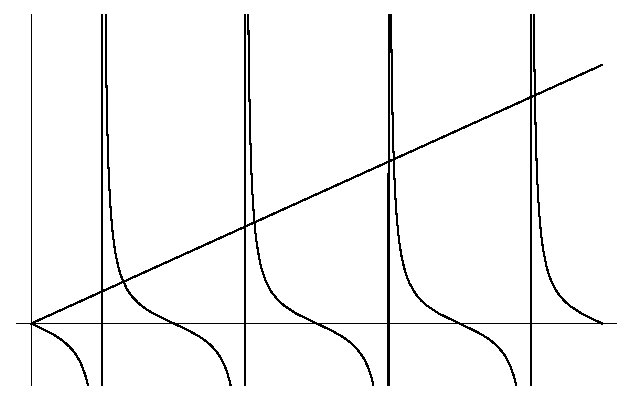
\includegraphics[width=0.4\textwidth]{ode/sturm/x_tanx}
    \end{center}
    \caption{The eigenvalues.}
    \label{x_tanx}
  \end{figure}

  From this we see that there are an infinite number of eigenvalues,
  $\lambda_1 < \lambda_2 < \lambda_3 < \cdots$.  In the limit as $n \to \infty$,
  $\lambda_n \to (n-1/2)\pi$.  The limit is approached from above.

  Now consider the eigenvalue problem
  \[
  y'' + y = \mu y  \quad y(0) = 0 \quad y(1) + y'(1) = 0.
  \]
  From above we see that the eigenvalues satisfy
  \[
  \sqrt{1 - \mu} = - \tan \left( \sqrt{1 - \mu} \right)
  \]
  and that there are an infinite number of eigenvalues.  For large $n$, 
  $\mu_n \approx 1 - (n - 1/2) \pi$.
  The eigenfunctions are 
  \[
  \phi_n = \sin \left( \sqrt{1 - \mu_n} x \right).
  \]

  To solve the inhomogeneous problem, we expand the solution and the 
  inhomogeneity in a series of the eigenfunctions.
  \begin{gather*}
    f = \sum_{n=1}^\infty f_n \phi_n, \quad 
    f_n = \frac{ \int_0^1 f(x) \phi_n(x) \,\dd x }{ \int_0^1 \phi_n^2(x) \,\dd x }
    \\
    y = \sum_{n=1}^\infty y_n \phi_n
  \end{gather*}
  We substitite the expansions into the differential equation to determine
  the coefficients.
  \begin{gather*}
    y'' + y = f
    \\
    \sum_{n=1}^\infty \mu_n y_n \phi_n = \sum_{n=1}^\infty f_n \phi_n
    \\
    \boxed{
      y = \sum_{n=1}^\infty \frac{f_n}{\mu_n} \sin \left( \sqrt{1 - \mu_n} x \right)
      }
  \end{gather*}
\end{Solution}












%% y'' +  y = f(x)  \quad y(0) = 0 \quad y(1) + y'(1) = 0.
\begin{Solution}
  \label{solution y''+y=f y+y'=0}
  Consider the eigenvalue problem
  \[
  y'' + y = \mu y  \quad y(0) = 0 \quad y(1) + y'(1) = 0.
  \]
  From Exercise~\ref{solution y''+ly=0 y+y'=0} we see that the eigenvalues 
  satisfy
  \[
  \sqrt{1 - \mu} = - \tan \left( \sqrt{1 - \mu} \right)
  \]
  and that there are an infinite number of eigenvalues.  For large $n$, 
  $\mu_n \approx 1 - (n - 1/2) \pi$.
  The eigenfunctions are 
  \[
  \phi_n = \sin \left( \sqrt{1 - \mu_n} x \right).
  \]

  To solve the inhomogeneous problem, we expand the solution and the 
  inhomogeneity in a series of the eigenfunctions.
  \begin{gather*}
    f = \sum_{n=1}^\infty f_n \phi_n, \quad 
    f_n = \frac{ \int_0^1 f(x) \phi_n(x) \,\dd x }{ \int_0^1 \phi_n^2(x) \,\dd x }
    \\
    y = \sum_{n=1}^\infty y_n \phi_n
  \end{gather*}
  We substitite the expansions into the differential equation to determine
  the coefficients.
  \begin{gather*}
    y'' + y = f
    \\
    \sum_{n=1}^\infty \mu_n y_n \phi_n = \sum_{n=1}^\infty f_n \phi_n
    \\
    \boxed{
      y = \sum_{n=1}^\infty \frac{f_n}{\mu_n} \sin \left( \sqrt{1 - \mu_n} x \right)
      }
  \end{gather*}
\end{Solution}













%% Mixed boundary condition.
\begin{Solution}
  \label{solution y''+ly=0 y'-y=0}
  First consider $\lambda = 0$.  The general solution is
  \[
  y = c_1 + c_2 x.
  \]
  $y = c x$ satisfies the boundary conditions.  Thus $\lambda = 0$ is an 
  eigenvalue.

  Now consider negative real $\lambda$.  The general solution is
  \[
  y = c_1 \cosh \left( \sqrt{-\lambda} x \right)
  + c_2 \sinh \left( \sqrt{-\lambda} x \right).
  \]
  The solution that satisfies the left boundary condition is
  \[
  y = c \sinh \left( \sqrt{-\lambda} x \right).
  \]
  For nontrivial solutions of the boundary value problem, there must be
  negative real solutions of 
  \[
  \sqrt{-\lambda} - \sinh \left( \sqrt{-\lambda} \right) = 0.
  \]
  Since $x = \sinh x$ has no nonzero real solutions, this equation has no 
  solutions for negative real $\lambda$.  There are no negative
  real eigenvalues.

  Finally consider positive real $\lambda$.  The general solution is
  \[
  y = c_1 \cos \left( \sqrt{\lambda} x \right)
  + c_2 \sin \left( \sqrt{\lambda} x \right).
  \]
  The solution that satisfies the left boundary condition is
  \[
  y = c \sin \left( \sqrt{\lambda} x \right).
  \]
  For nontrivial solutions of the boundary value problem, there must be
  positive real solutions of 
  \[
  \sqrt{\lambda} - \sin \left( \sqrt{\lambda} \right) = 0.
  \]
  Since $x = \sin x$ has no nonzero real solutions, this equation has no 
  solutions for positive real $\lambda$.  There are no positive
  real eigenvalues.

  There is only one real eigenvalue, $\lambda = 0$, with corresponding 
  eigenfunction $\phi = x$.

  The difficulty with the boundary conditions, $y(0) = 0$, $y'(0) - y(1) = 0$
  is that the problem is not self-adjoint.  
  We demonstrate this by showing that the problem does
  not satisfy Green's identity.  Let $u$ and $v$ be two functions that 
  satisfy the boundary conditions, but not necessarily the differential 
  equation.
  \begin{align*}
    \langle u, L[v] \rangle - \langle L[u], v \rangle
    &= \langle u, v'' \rangle - \langle u'', v \rangle \\
    &= \left[ u v' \right]_0^1 - \langle u', v' \rangle - \langle u', v' \rangle 
    - \left[ u' v \right]_0^1 + \langle u', v' \rangle - \langle u', v' \rangle \\
    &= u(1) v'(1) - u'(1) v(1)
  \end{align*}
  Green's identity is not satisfied,
  \[
  \langle u, L[v] \rangle - \langle L[u], v \rangle \neq 0;
  \]
  The problem is not self-adjoint.
\end{Solution}











%% Rayleigh quotient for Bessel equation.
\begin{Solution}
  \label{solution y''+1xy'+ly=0}
  First we write the equation in formally self-adjoint form,
  \[
  L[y] \equiv 
  (x y')' = - \lambda x y, \quad 
  |y(0)| < \infty, \quad y(1) = 0.
  \]
  Let $\lambda$ be an eigenvalue with corresponding eigenfunction $\phi$.
  We derive the Rayleigh quotient for $\lambda$.
  \begin{gather*}
    \langle \phi, L[\phi] \rangle = \langle \phi, - \lambda x \phi \rangle \\
    \langle \phi, (x \phi')' \rangle = -\lambda \langle \phi, x \phi \rangle \\
    \left[ \phi x \phi' \right]_0^1 - \langle \phi', x \phi' \rangle 
    = -\lambda \langle \phi, x \phi \rangle \\
    \intertext{We apply the boundary conditions and solve for $\lambda$.}
    \boxed{
      \lambda = \frac{ \langle \phi', x \phi' \rangle }{ \langle \phi, x \phi \rangle }
      }
  \end{gather*}
  The Bessel equation of the first kind and order zero satisfies the problem,
  \[
  y'' + \frac{1}{x} y' + y = 0, \quad
  |y(0)| < \infty, \quad y(r) = 0,
  \]
  where $r$ is a positive root of $J_0(x)$.  We make the change of variables
  $\xi = x/r$, $u(\xi) = y(x)$ to obtain the problem
  \[
  \frac{1}{r^2} u'' + \frac{1}{r \xi} \frac{1}{r} u' + u = 0, \quad
  |u(0)| < \infty, \quad u(1) = 0,
  \]
  \[
  u'' + \frac{1}{\xi} u' + r^2 u = 0, \quad
  |u(0)| < \infty, \quad u(1) = 0.
  \]
  Now $r^2$ is the eigenvalue of the problem for $u(\xi)$.  From the Rayleigh
  quotient, the minimum eigenvalue obeys the inequality
  \[
  r^2 \leq \frac{ \langle \phi', x \phi' \rangle }{ \langle \phi, x \phi \rangle },
  \]
  where $\phi$ is any test function that satisfies the boundary 
  conditions.  Taking $\phi = 1-x$ we obtain,
  \[
  r^2 \leq \frac{ \int_0^1 (-1) x (-1) \,\dd x }{ \int_0^1 (1-x)x(1-x)\,\dd x } = 6,
  \]
  \[
  \boxed{
    r \leq \sqrt{6}
    }
  \]
  Thus the smallest zero of $J_0(x)$ is less than or equal to 
  $\sqrt{6} \approx 2.4494$.  (The smallest zero of $J_0(x)$ is approximately
  $2.40483$.)
\end{Solution}












%% y'' + \lambda q(z) y = 0, \qquad y(0) = y(\pi) = 0
\begin{Solution}
  \label{solution y''+lqy=0}
  We assume that $0 < l < \pi$.

  Recall that the solution of a second order differential equation with
  piecewise continuous coefficient functions is piecewise $C^2$.  
  This means that the solution is $C^2$ except for a finite number of points
  where it is $C^1$.

  First consider the case $\lambda = 0$.  A set of linearly independent
  solutions of the differential equation is $\{1,z\}$.  The solution which
  satisfies $y(0) = 0$ is $y_1 = c_1 z$. The solution which
  satisfies $y(\pi) = 0$ is $y_2 = c_2 (\pi-z)$. There is a solution for
  the problem if there are there are values of $c_1$ and $c_2$ such 
  that $y_1$ and $y_2$ have the same position and slope at $z = l$.
  \begin{gather*}
    y_1(l) = y_2(l), \quad y_1'(l) = y_2'(l) \\
    c_1 l = c_2 (\pi - l), \quad c_1 = -c_2 
  \end{gather*}
  Since there is only the trivial solution, $c_1 = c_2 = 0$, $\lambda = 0$ is
  not an eigenvalue.




  Now consider $\lambda \neq 0$.  For $0 \leq z \leq l$ a set of linearly
  independent solutions is
  \[
  \left\{ \cos( \sqrt{a \lambda} z ), \sin( \sqrt{a \lambda} z ) \right\}.
  \]
  The solution which satisfies $y(0) = 0$ is
  \[
  y_1 = c_1 \sin( \sqrt{a \lambda} z ).
  \]
  For $l < z \leq \pi$ a set of linearly
  independent solutions is
  \[
  \left\{ \cos( \sqrt{b \lambda} z ), \sin( \sqrt{b \lambda} z ) \right\}.
  \]
  The solution which satisfies $y(\pi) = 0$ is
  \[
  y_2 = c_2 \sin( \sqrt{b \lambda} (\pi - z) ).
  \]
  $\lambda \neq 0$ is an eigenvalue if there are nontrivial solutions of
  \begin{gather*}
    y_1(l) = y_2(l), \quad y_1'(l) = y_2'(l) \\
    c_1 \sin( \sqrt{a \lambda} l ) = c_2 \sin( \sqrt{b \lambda} (\pi - l) ), \quad
    c_1 \sqrt{a \lambda} \cos( \sqrt{a \lambda} l ) 
    = - c_2 \sqrt{b \lambda} \cos( \sqrt{b \lambda} (\pi - l) )
  \end{gather*}
  We divide the second equation by $\sqrt(\lambda)$ since $\lambda \neq 0$
  and write this as a linear algebra problem.
  \[
  \begin{pmatrix}
    \sin( \sqrt{a \lambda} l ) & - \sin( \sqrt{b \lambda} (\pi - l) ) \\
    \sqrt{a} \cos( \sqrt{a \lambda} l ) & 
    \sqrt{b} \sin( \sqrt{b \lambda} (\pi - l) )
  \end{pmatrix}
  \begin{pmatrix}
    c_1 \\
    c_2
  \end{pmatrix}
  =
  \begin{pmatrix}
    0 \\
    0
  \end{pmatrix}
  \]
  This system of equations has nontrivial solutions if and only if the 
  determinant of the matrix is zero.
  \[
  \sqrt{b} \sin( \sqrt{a \lambda} l ) \sin( \sqrt{b \lambda} (\pi - l) )
  + \sqrt{a} \cos( \sqrt{a \lambda} l )\sin( \sqrt{b \lambda} (\pi - l) ) = 0
  \]
  We can use trigonometric identities to write this equation as
  \[
  \boxed{
    (\sqrt{b} - \sqrt{a}) \sin \left( \sqrt{\lambda} 
      ( l \sqrt{a} - (\pi - l) \sqrt{b} ) \right)
    + (\sqrt{b} + \sqrt{a}) \sin \left( \sqrt{\lambda} 
      ( l \sqrt{a} + (\pi - l) \sqrt{b} ) \right) = 0
    }
  \]
  Clearly this equation has an infinite number of solutions for real, positive
  $\lambda$.  However, it is not clear that this equation does not have 
  non-real solutions. In order to prove that, we will show that the 
  problem is self-adjoint.  Before going on to that we note that
  the eigenfunctions have the form
  \[
  \boxed{
    \phi_n(z) = \begin{cases}
      \sin \left(\sqrt{a \lambda_n} z \right) & 0 \leq z \leq l \\
      \sin \left(\sqrt{b \lambda_n} (\pi-z) \right) & l < z \leq \pi.
    \end{cases}
    }
  \]

  Now we prove that the problem is self-adjoint.  We consider the class of 
  functions which are $C^2$ in $(0 \ldots \pi)$ except at the interior point
  $x = l$ where they are $C^1$ and which satisfy the boundary conditions
  $y(0)= y(\pi) = 0$.  Note that the differential operator is not 
  defined at the point $x = l$.  Thus Green's identity, 
  \[
  \langle u | q | L v \rangle = \langle L u | q | v \rangle
  \]
  is not well-defined. To remedy this we must define a new inner product.
  We choose
  \[
  \langle u | v \rangle \equiv \int_0^l \overline{u} v \,\dd x 
  + \int_l^\pi \overline{u} v \,\dd x.
  \]
  This new inner product does not require differentiability at the point $x = l$.

  The problem is self-adjoint if Green's indentity is satisfied.
  Let $u$ and $v$ be elements of our class of functions.
  In addition to the boundary conditions, we will use the fact that 
  $u$ and $v$ satisfy $y(l^-) = y(l^+)$ and $y'(l^-) = y'(l^+)$.
  \begin{align*}
    \langle v | L u \rangle 
    &= \int_0^l \overline{v} u'' \,\dd x + \int_l^\pi \overline{v} u'' \,\dd x \\
    &= \left[ \overline{v} u' \right]_0^l - \int_0^l \overline{v}' u' \,\dd x 
    + \left[ \overline{v} u' \right]_l^\pi - \int_l^\pi \overline{v}' u' \,\dd x \\
    &= \overline{v}(l) u'(l) - \int_0^l \overline{v}' u' \,\dd x 
    - \overline{v}(l) u'(l) - \int_l^\pi \overline{v}' u' \,\dd x \\
    &= - \int_0^l \overline{v}' u' \,\dd x 
    - \int_l^\pi \overline{v}' u' \,\dd x \\
    &= - \left[ \overline{v}' u \right]_0^l + \int_0^l \overline{v}'' u \,\dd x 
    - \left[ \overline{v}' u \right]_l^\pi + \int_l^\pi \overline{v}'' u \,\dd x \\
    &= - \overline{v}'(l) u(l) + \int_0^l \overline{v}'' u \,\dd x 
    + \overline{v}'(l) u(l) + \int_l^\pi \overline{v}'' u \,\dd x \\
    &= \int_0^l \overline{v}'' u \,\dd x + \int_l^\pi \overline{v}'' u \,\dd x \\
    &= \langle L v | L u \rangle 
  \end{align*}
  The problem is self-adjoint.  Hence the eigenvalues are real.
  There are an infinite number of positive, real eigenvalues $\lambda_n$.
\end{Solution}







%% Find conditions on the smooth real functions $p(x)$, $q(x)$, $r(x)$ and 
\begin{Solution}
  \label{solution pv''''-qv''+rv=lsv}
  \begin{enumerate}
    %%
    %%
  \item
    Let $v$ be an eigenfunction with the eigenvalue $\lambda$.
    We start with the differential equation and then take the inner product 
    with $v$.
    \begin{gather*}
      (p v'')'' - (q v')' + r v = \lambda s v \\
      \langle v, (p v'')'' - (q v')' + r v \rangle = \langle v, \lambda s v \rangle \\
      \intertext{We use integration by parts and utilize the homogeneous 
        boundary conditions.}
      \left[ v (p v'')' \right]_a^b - \langle v', (p v'')' \rangle
      - \left[ v q v' \right]_a^b + \langle v', q v' \rangle
      + \langle v, r v \rangle = \lambda \langle v, s v \rangle \\
      - \left[ v' p v'' \right]_a^b + \langle v'', p v'' \rangle + \langle v', q v' \rangle
      + \langle v, r v \rangle = \lambda \langle v, s v \rangle \\
      \lambda = \frac{ \langle v'', p v'' \rangle + \langle v', q v' \rangle + \langle v, r v \rangle }
      { \langle v, s v \rangle }
    \end{gather*}
    We see that if $p,q,r,s \geq 0$ then the eigenvalues will be positive.
    (Of course we assume that $p$ and $s$ are not identically zero.)
    %%
    %%
  \item
    First we prove that this problem is self-adjoint.  Let $u$ and $v$ be functions
    that satisfy the boundary conditions, but do not necessarily satsify 
    the differential equation.
    \begin{align*}
      \langle v, L[u] \rangle - \langle L[v], u \rangle
      &= \langle v, (p u'')'' - (q u')' + r u \rangle
      - \langle (p v'')'' - (q v')' + r v, u \rangle \\
      \intertext{Following our work in part (a) we use integration by parts to 
        move the derivatives.}
      &= \left( \langle v'', p u'' \rangle + \langle v', q u' \rangle 
        + \langle v, r u \rangle \right)
      - \left( \langle p v'', u'' \rangle + \langle q v', u' \rangle 
        + \langle r v, u \rangle \right) \\
      &= 0
    \end{align*}
    This problem satisfies Green's identity,
    \[
    \langle v, L[u] \rangle - \langle L[v], u \rangle = 0,
    \]
    and is thus self-adjoint.

    Let $v_k$ and $v_m$ be eigenfunctions corresponding to the distinct 
    eigenvalues $\lambda_k$ and $\lambda_m$.  We start with Green's identity.
    \begin{align*}
      \langle v_k, L[v_m] \rangle - \langle L[v_k], v_m \rangle = 0 \\
      \langle v_k, \lambda_m s v_m \rangle - \langle \lambda_k s v_k, v_m \rangle = 0 \\
      (\lambda_m - \lambda_k) \langle v_k, s v_m \rangle = 0 \\
      \langle v_k, s v_m \rangle = 0 
    \end{align*}
    The eigenfunctions are orthogonal with respect to the weighting function $s$.
    %%
    %%
  \item
    From part (a) we know that there are only positive eigenvalues.
    The general solution of the differential equation is
    \[
    \phi = c_1 \cos( \lambda^{1/4} x ) + c_2 \cosh( \lambda^{1/4} x )
    + c_3 \sin( \lambda^{1/4} x ) + c_4 \sinh( \lambda^{1/4} x ).
    \]
    Applying the condition $\phi(0) = 0$ we obtain
    \[
    \phi = c_1 ( \cos( \lambda^{1/4} x ) - \cosh( \lambda^{1/4} x ) )
    + c_2 \sin( \lambda^{1/4} x ) + c_3 \sinh( \lambda^{1/4} x ).
    \]
    The condition $\phi''(0) = 0$ reduces this to
    \[
    \phi = c_1 \sin( \lambda^{1/4} x ) + c_2 \sinh( \lambda^{1/4} x ).
    \]
    We substitute the solution into the two right boundary conditions.
    \begin{align*}
      c_1 \sin( \lambda^{1/4} ) + c_2 \sinh( \lambda^{1/4} ) &= 0 \\
      - c_1 \lambda^{1/2} \sin( \lambda^{1/4} ) 
      + c_2 \lambda^{1/2} \sinh( \lambda^{1/4} ) &= 0 
    \end{align*}
    We see that $\sin( \lambda^{1/4} ) = 0$.  The eigenvalues and eigenfunctions
    are
    \[
    \lambda_n = (n \pi)^4, \quad \phi_n = \sin( n \pi x ), \quad n \in \mathbb{N}.
    \]
  \end{enumerate}
\end{Solution}



\raggedbottom
}
